%%%%%%%%%%%%%%%%%%%%%%%%%%%%%%%%%%%%%%%%%
% Beamer Presentation
% LaTeX Template
% Version 1.0 (10/11/12)
%
% This template has been downloaded from:
% http://www.LaTeXTemplates.com
%
% License:
% CC BY-NC-SA 3.0 (http://creativecommons.org/licenses/by-nc-sa/3.0/)
%
%%%%%%%%%%%%%%%%%%%%%%%%%%%%%%%%%%%%%%%%%

%----------------------------------------------------------------------------------------
%	PACKAGES AND THEMES
%----------------------------------------------------------------------------------------

\documentclass{beamer}
\mode<presentation> {
\usetheme{Madrid}
}
\usepackage{url}
\usepackage{lmodern}
\usepackage{graphicx}
\usepackage{booktabs}

% for mathematics
\usepackage{amsmath}
\usepackage{amsthm}

%----------------------------------------------------------------------------------------
%	TITLE PAGE
%----------------------------------------------------------------------------------------

\title[Financial mathematics with Python]{UROPS Project Presentation 3} % The short title appears at the bottom of every slide, the full title is only on the title page

\author{Wang Zexin} % Your name
\institute[NUS]
{
Variance Reduction Techniques\\
of Monte Carlo methods in Financial Engineering\\[3mm]
\medskip
\textit{Quantitative Finance\\
National University of Singapore\\}
}
\date{\today}

\begin{document}
%----------------------------------------------------------------------------------------
%	TITLE PAGE
%----------------------------------------------------------------------------------------
\begin{frame}
\titlepage
\end{frame}

%----------------------------------------------------------------------------------------
%	TABLE OF CONTENTS
%----------------------------------------------------------------------------------------

%------------------------------------------------
\begin{frame}
\frametitle{Today's Agenda}
\tableofcontents
\end{frame}

%------------------------------------------------
\begin{frame}
\frametitle{Changes due to different Python version}
We are using Python 3.6 while the version in the book is Python 2.7\\
So here is a list of items to change\\[2mm]
\begin{itemize}
	\item print x now becomes print(x)
	\item dict.iteritems() now becomes dict.items()
	\item xrange now becomes range
	\item lambda (k, v) : (v, k) is no longer available
	\item instead we can only use: lambda x : (x[1], x[0])
	\item x / 2 is float division, while x // 2 is integer division
\end{itemize}
\end{frame}

\section{Variance Reduction Techniques} %------------------------------------------------

\subsection{Control Variates}

%------------------------------------------------
\begin{frame}
\frametitle{Control Variates - Mathematics}
Our aim is to estimate $\mathrm{E}[Y_{i}]$ \\
Under simulation, we use : $$\bar{Y} = \frac{1}{n} \sum_{i=1}^{n} Y_{i}$$ (unbiased estimate)\\
Now we introduce a new variable $X$, with realizations $X_{i}$, for i from 1 to n\\
Define $Y_{i}(\lambda) = Y_{i} - \lambda (X_{i} - \mathrm{E}(X))$
$$\bar{Y}(\lambda) = \bar{Y} - \lambda (\bar{X} - \mathrm{E}(X)) = \frac{1}{n} \sum_{i=1}^{n} [Y_{i} - \lambda (X_{i} - \mathrm{E}(X))]$$
\end{frame}

%------------------------------------------------
\begin{frame}
\frametitle{Control Variates - Unbiasedness and Consistency}
The new estimate $\bar{Y}(\lambda)$ is unbiased and consistent.\\[5mm]
Unbiasedness: $$\mathrm{E}(\bar{Y}(\lambda)) = \mathrm{E}[\bar{Y} - \lambda(\bar{X} - \mathrm{E}(X))] = \mathrm{E}(\bar{Y}) - \lambda(\mathrm{E}(\bar{X}) - \mathrm{E}(X)) = \mathrm{E}(Y) $$
\begin{equation*}
\begin{split}
Consistency: \lim_{n\to\infty} \frac{1}{n}\sum_{i=1}^{n} Y_{i}(\lambda) 
&=\lim_{n\to\infty} \frac{1}{n}\sum_{i=1}^{n} [Y_{i} - \lambda (X_{i} - \mathrm{E}(X))] \\
&= \mathrm{E}[Y - \lambda(X-\mathrm{E}(X))] \\
&= \mathrm{E}(Y) \\
\end{split}
\end{equation*}
\end{frame}

%------------------------------------------------
\begin{frame}
\frametitle{Control Variates - Controlling Variance of estimate}
\begin{equation*}
\begin{split}
\mathrm{Var}[Y_{i}(\lambda)]
&=\mathrm{Var} [Y_{i} - \lambda(X_{i} - \mathrm{E}(X))] \\
&= \mathrm{Var}[Y_{i} - \lambda X_{i}] \\
&= \mathrm{Var}(Y_{i}) + \lambda^{2}\mathrm{Var}(X_{i}) - 2\lambda\mathrm{Cov}(X_{i}, Y_{i}) \\
&= \sigma_{Y}^{2} + \lambda^{2}\sigma_{X}^{2}-2\lambda\sigma_{X}\sigma_{Y}\rho_{XY}\\
\end{split}
\end{equation*}
\begin{center}
In order to find the minimum variance by varying $\lambda$\\[2mm]
Set $\frac{\partial \mathrm{Var}[Y_{i}(\lambda)]}{\partial \lambda} = 2\lambda \sigma_{X}^{2} - 2\sigma_{X}\sigma_{Y}\rho_{XY}$ to 0:
\end{center}
$$ \lambda^{*} = \frac{2\sigma_{X}\sigma_{Y}\rho_{XY}}{2\sigma_{X}^{2}} = \frac{\sigma_{X}\sigma_{Y}\rho_{XY}}{\sigma_{X}^{2}} = \frac{\mathrm{Cov}(X,Y)}{\mathrm{Var}(X)}$$
\end{frame}

%------------------------------------------------
\begin{frame}
\frametitle{Control Variates - Controlling Variance of estimate}
Compare the new variance with the old:
\begin{equation*}
\begin{split}
\frac{\mathrm{Var} [Y_{i} - \lambda^{*}(X_{i} - \mathrm{E}(X))]}{\mathrm{Var}(Y)}
&=\frac{\sigma_{Y}^{2} + {\lambda^{*}}^{2}\sigma_{X}^{2}-2\lambda^{*}\sigma_{X}\sigma_{Y}\rho_{XY}}{\sigma_{Y}^{2}} \\
&=1+\frac{\frac{\mathrm{Var}(X)(\mathrm{Cov}(X,Y))^{2}}{(\mathrm{Var}(X))^{2}}-\frac{2(\mathrm{Cov}(X,Y))^{2}}{\mathrm{Var}(X)}}{\sigma_{Y}^{2}}\\
&=1+\frac{\frac{\sigma_{X}^{4}\sigma_{Y}^{2}\rho_{XY}^{2}}{\sigma_{X}^{4}}-\frac{2\sigma_{X}^{2}\sigma_{Y}^{2}\rho_{XY}^{2}}{\sigma_{X}^{2}}}{\sigma_{Y}^{2}}\\
&=1+\frac{\sigma_{Y}^{2}\rho_{XY}^{2}-2\sigma_{Y}^{2}\rho_{XY}^{2}}{\sigma_{Y}^{2}}\\
&=1-\rho_{XY}^{2}\\
\end{split}
\end{equation*}
Conclusion from the theoretical results:\\
The stronger the correlation, the better the reduction in variance.
\end{frame}

%------------------------------------------------
\begin{frame}
\frametitle{Choices of Control Variates}
We can use several different random variables as control variates.
\begin{itemize}
	\item Underlying asset prices
	\item Tractable options
	\item Bond prices
	\item Tractable dynamics
\end{itemize}
\end{frame}

%------------------------------------------------
\begin{frame}
\frametitle{Control Variates - estimate for $\lambda^{*}$}
In the case that it is not feasible to calculate using the probability distribution of $X$ and $Y$, we should work $\lambda^{*}$ out as an estimate.
$$ \hat{\lambda}^{*} = \frac{\mathrm{Cov}(X,Y)}{\mathrm{Var}(X)} \approx \frac{\sum_{i=1}^{n}(X_{i}-\bar{X})(Y_{i}-\bar{Y})}{\sum_{i=1}^{n}(X_{i}-\bar{X})^{2}}$$
\end{frame}

%------------------------------------------------
\begin{frame}
\frametitle{Implementation of Algorithm in pseudocode}
\begin{itemize}
	\item // pilot simulation to obtain correlation
	\item for i = 1 to n
	\item \quad $generate(X_{i}, Y_{i})$
	\item end for
	\item computer $\lambda^{*} = \frac{\mathrm{Cov}(X,Y)}{\mathrm{Var}(X)}$
	\item for i = 1 to n
	\item \quad $generate(X_{i}, Y_{i})$
	\item \quad set ${Y}_{i}(\lambda) = Y_{i} + \lambda^{*}(X_{i}-\mathrm{E}[X])$
	\item end for
	\item Estimate : $\bar{Y}(\lambda) = \frac{1}{n} \sum_{i=1}^{n} {Y}_{i}(\lambda)$
	\item $\hat{\sigma}_{n, Y_{\lambda}}^{2} = \frac{1}{n-1} \sum({Y}_{i}(\lambda)-\bar{Y}(\lambda))^{2}$
	\item $100(1-\alpha)\% C.I. = [\bar{Y}(\lambda) - \mathcal{Z}_{1-\alpha/2} \frac{\hat{\sigma}_{n, Y_{\lambda}}}{\sqrt{n}}, \bar{Y}(\lambda) + \mathcal{Z}_{1-\alpha/2} \frac{\hat{\sigma}_{n, Y_{\lambda}}}{\sqrt{n}}] $
\end{itemize}
\end{frame}

%------------------------------------------------
\begin{frame}
\frametitle{Underlying asset prices for european call payoff}
The underlying asset prices provide a source of control variates for its natural correlation with the derivative payoff.\\
The control variate estimator is formed like this:
$$ \frac{1}{n}\sum_{i=1}^{n}(Y_{i}-\lambda[S_{i}(T)-e^{rT}S(0)])$$
For European Call option, $Y = e^{-rT}(S(T)-K)^{+}$.
However, one problem arises: as the strike price goes higher, the correlation of the underlying asset prices and the payoff decreases, this diminishes the effect of control variates upon variance reduction.
\end{frame}

%------------------------------------------------
\begin{frame}
\frametitle{Underlying asset prices for european call payoff (bug fixed)}
\begin{figure}[H]
	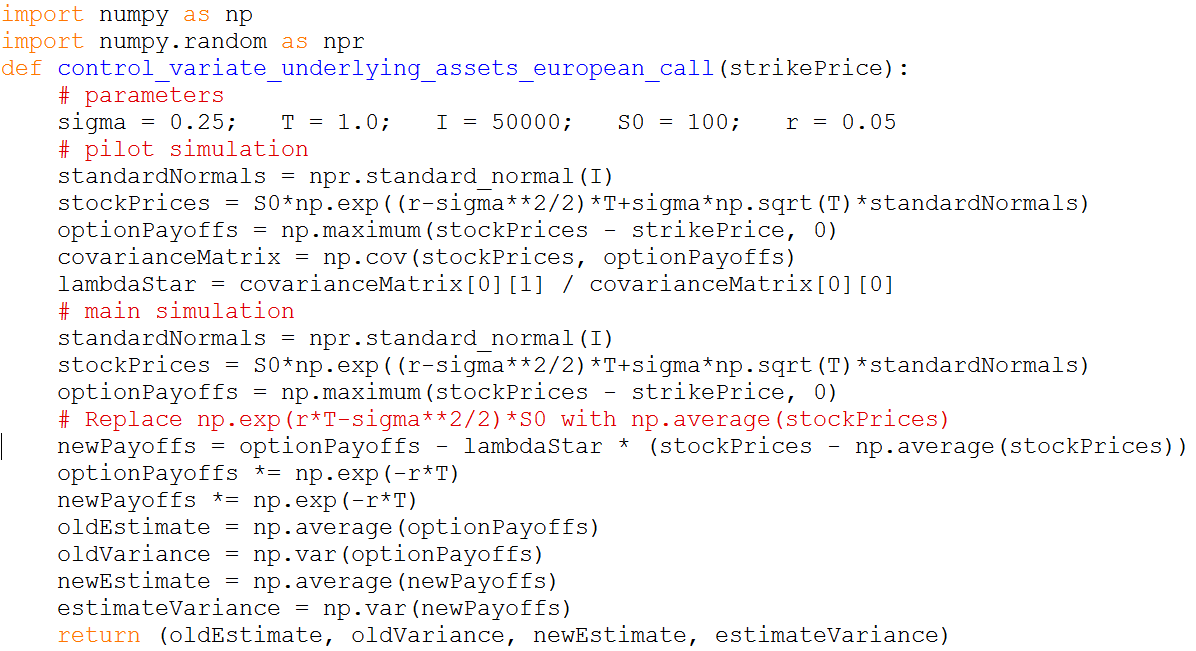
\includegraphics[scale=0.38]{control_variate_european_call_underlying_asset_prices.png}
\end{figure}
\end{frame}

%------------------------------------------------
\begin{frame}
\frametitle{Underlying asset prices for european call payoff (bug fixed)}
\begin{figure}[H]
	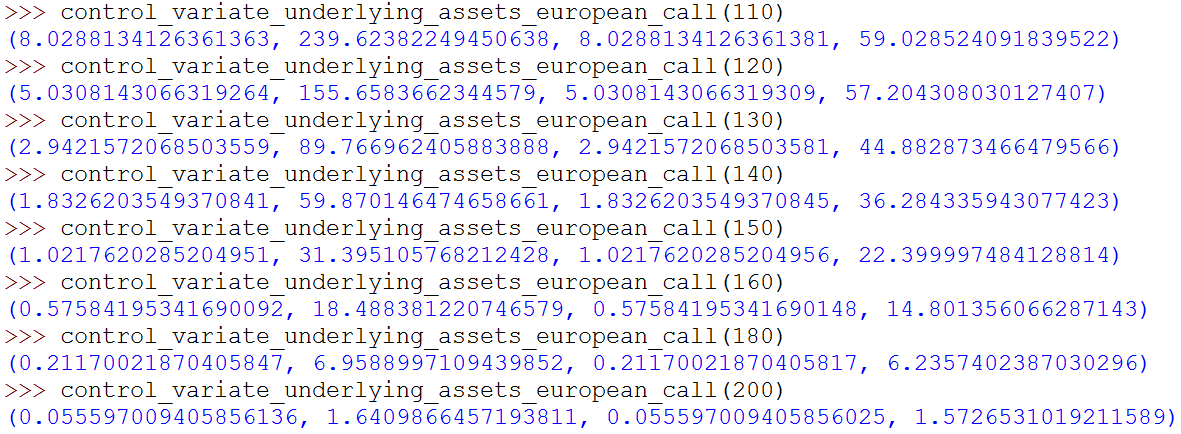
\includegraphics[scale=0.38]{control_variate_european_call_underlying_asset_prices_test.png}
\end{figure}
From the output, we can see that as time goes, the proportion of variance reduced from including underlying asset prices as control variates decreases. However, as the proportion of variance reduction drops, the initial variance is also decreasing. Hence we can still comment that underlying asset price can serve as a good choice of control variate.
\end{frame}

%------------------------------------------------
\begin{frame}
\frametitle{Tractable options for european call payoff}
The payoff of other tractable options may also provide a source of control variates for its natural correlation with the derivative payoff.\\
The control variate estimator is formed like this:
$$ \frac{1}{n}\sum_{i=1}^{n}(Y_{i}-\lambda[(K^{\prime}-S_{i}(T))^{+}-\mathrm{E}((K^{\prime}-S(T))^{+})])$$
For European Call option, $Y = e^{-rT}(S(T)-K)^{+}$.\\
Here we are using European Put option payoff as the control variates, with $K^{\prime}$ being the put option strike price and $(K^{\prime}-S(T))^{+}$ being the put option payoff.\\ The problem is that we do not know which strike price may give the strongest correlation between these two option payoffs, so I shall start with experimenting on some of the potential candidates.
\end{frame}

%------------------------------------------------
\begin{frame}
\frametitle{Tractable options for european call payoff - programme}
\begin{figure}[H]
	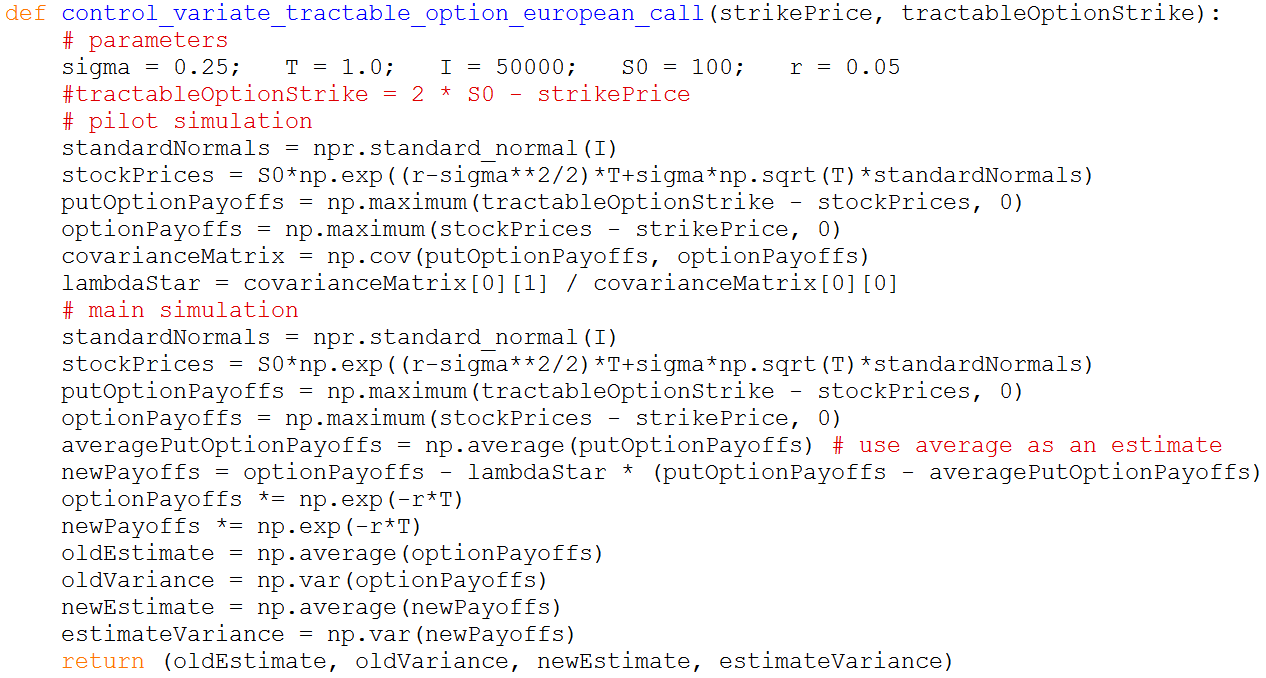
\includegraphics[scale=0.36]{control_variate_european_call_put_option.png}
\end{figure}
\end{frame}

%------------------------------------------------
\begin{frame}
\frametitle{Tractable options for european call payoff - test}
\begin{figure}[H]
	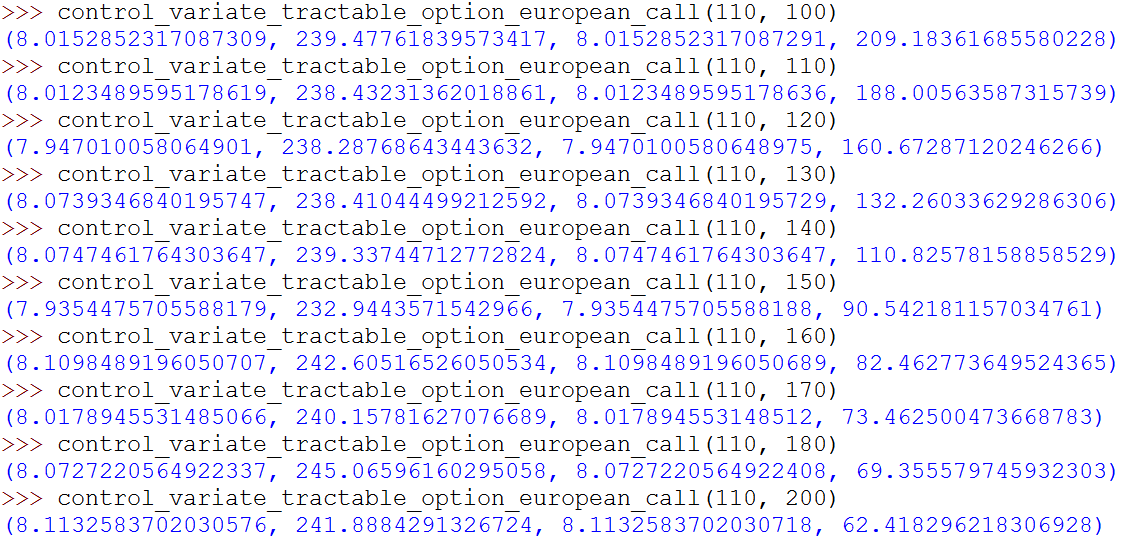
\includegraphics[scale=0.36]{control_variate_european_call_put_option_test1.png}
\end{figure}
When strike price is low, the increase in the strike price of put option will cause a larger proportion of reduction in variance.  However, as the strike price increases, the payoffs is becoming more similar to stock prices, and eventually it can only achieve the same reduction in variance as compared to using underlying asset prices when the strike is infinitely large.
\end{frame}

%------------------------------------------------
\begin{frame}
\frametitle{Tractable options for european call payoff - test}
\begin{figure}[H]
	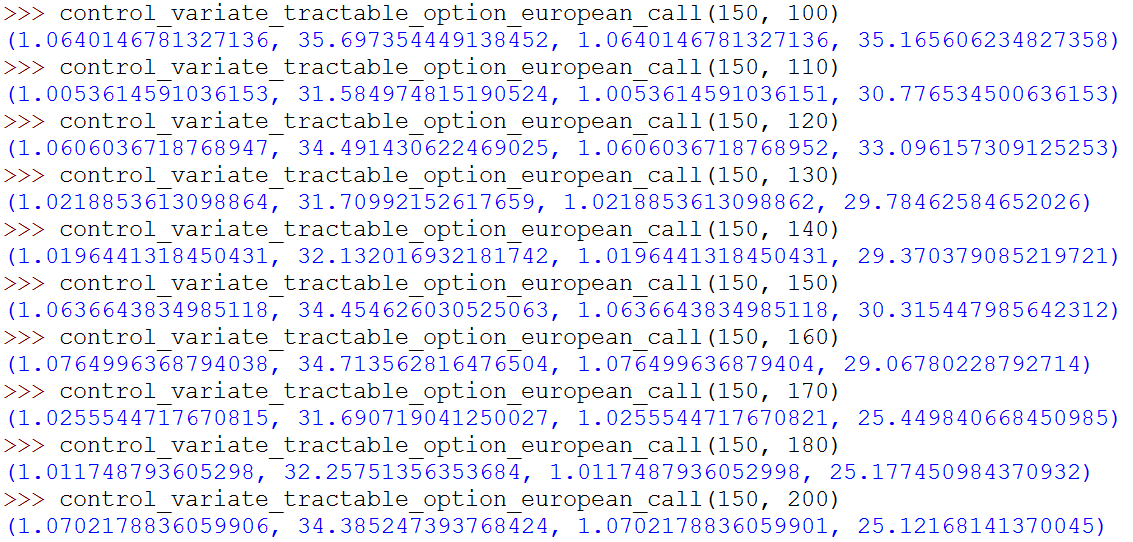
\includegraphics[scale=0.38]{control_variate_european_call_put_option_test2.png}
\end{figure}
When the strike price of call option is higher, the increase in the strike price of put option will cause a larger proportion of reduction in variance generally. Still there is one point which is the strike price of the call, where the reduction in variance seems to achieve  its minimum.
\end{frame}

%------------------------------------------------
\begin{frame}
\frametitle{Tractable options for european call payoff - test}
Hence, this method of underlying variates using Tractable options can only work at most as good as the method using underlying asset prices as control variates.
\end{frame}

\subsection{Stratified Sampling}

%------------------------------------------------
\begin{frame}
\frametitle{Stratified Sampling - Mathematics}
Stratified sampling refers broadly to any sampling mechanism that constrains
the fraction of observations drawn from specific subsets (or strata) of the
sample space. \\
Goal: estimate $\mathrm{E}[Y]$, $Y \in \mathbb{R}$\\
Dividing the sample space into K parts, with $A_{1}, \dots ,A_{K}$ being disjoint subsets of the real line for which $\mathrm{P}(Y \in \cup_{i}A_{i}) = 1$. \\
Then by the Bayes$^{\prime}$ Theorem,
$$ \mathrm{E}[Y] = \sum_{i=1}^{K}\mathrm{P}(Y \in A_{i})\mathrm{E}[Y|Y \in A_{i}] = \sum_{i=1}^{K}p_{i}\mathrm{E}[Y|Y \in A_{i}] $$
\end{frame}

%------------------------------------------------
\begin{frame}
\frametitle{Stratified Sampling - Mathematics}
Simplest case: proportional sampling, ensuring $p_{i} = \mathrm{P}(Y \in A_{i})$, the fraction of observations drawn from stratum $A_{i}$ exactly matches theoretical probability.\\
Unbiased estimator of $\mathrm{E}(Y)$ is provided by:\\
$$\hat{Y} = \sum_{i=1}^{K} p_{i} \frac{1}{n_{i}} \sum_{j=1}^{n_{i}} Y_{ij} = \frac{1}{n} \sum_{i=1}^{K} \sum_{j=1}^{n_{i}} Y_{ij}$$
$$ \mathrm{E}[\hat{Y}] = \mathrm{E}[\sum_{i=1}^{K} p_{i} \frac{1}{n_{i}} \sum_{j=1}^{n_{i}} Y_{ij}] = \sum_{i=1}^{K}\mathrm{P}(Y \in A_{i})\mathrm{E}[Y|Y \in A_{i}] = \mathrm{E}[Y]$$
\end{frame}

%------------------------------------------------
\begin{frame}
\frametitle{Stratified Sampling - Mathematics}
Simplest case: proportional sampling, ensuring $p_{i} = \mathrm{P}(Y \in A_{i})$, the fraction of observations drawn from stratum $A_{i}$ exactly matches theoretical probability.\\
We shall generate a stratification variable $X$ which take values in the union of the disjoint sets $A_{i}$s. As supposedly the values of $X$ are high correlated to the values of $Y$, in many cases, $Y$ is a function of X. For example, if $Y$ is the discounted payoff of European call option, $X$ can be the discrete path of underlying asset prices.\\
\end{frame}

%------------------------------------------------
\begin{frame}
\frametitle{Stratified Sampling - Algorithm}
Let $X$ be the discrete path of underlying asset prices, with $Y$ being the European call payoff discounted to time 0. If $X$ has $k$ discrete prices on one path, $\Omega \in \mathbb{R}^{k}$ is the sample space for the $X_{i}$s, where $\Omega = \cup_{i} A_{i}$ is the union of disjoint sets.\\
Here for the purpose of stratified sampling we should satisfy two conditions:
\begin{itemize}
	\item $\mathbb{P}(X \in A_{i})$ can be easily computed.
	\item $(Y | X \in A_{i})$ Given $X \in A_{i}$, $Y$ can be easily generated.
\end{itemize}
In order to further simplify the trouble of dividing $\Omega$ into disjoint subsets, we are going to use the stock prices half way as a condition to fully determine the distributions of $A_{i}$. The possible stock prices at time $\frac{T}{2}$ will be generated based on the Geometric Brownian Motion of the underlying stock prices. Given we are going to produce $n$ equal probable subsets of $\Omega$, the standard normal distribution can be sliced into $n$ pieces to provide sources of generation.
\end{frame}

%------------------------------------------------
\begin{frame}
\frametitle{Stratified Sampling - Algorithm}
If the standard normal distribution is going to be splitted into 50 parts, with each starting from quantile 0\% to quantile 2\%, quantile 2\% to quantile 4\%, \dots, quantile 98\% to quantile 100\%, we shall use their middle point in quantile to generate expectations of stock prices half way, namely quantile 1\%, quantile 3\%, \dots, quantile 99\%.\\
The next part of algorithm is to use the GBM formula to calculate the 50 expectations of the stock prices at time $\frac{T}{2}$.
$$S_{T} = S_{0}\exp\{(r-\frac{1}{2}\sigma^{2})T + \sigma\sqrt{T}z_{\alpha_{i}}\}$$
where $z_{\alpha_{i}}$ is the quantile of standard normal distribution at $(2i-1)\%$
With the expectations at these points, we can go on to generate for every group $\frac{\mathrm{I}}{50}$ number of stock prices at time $T$, and calculate the corresponding European call payoffs.
\end{frame}

%------------------------------------------------
\begin{frame}
\frametitle{Stratified Sampling - Implementation}
\begin{figure}[H]
	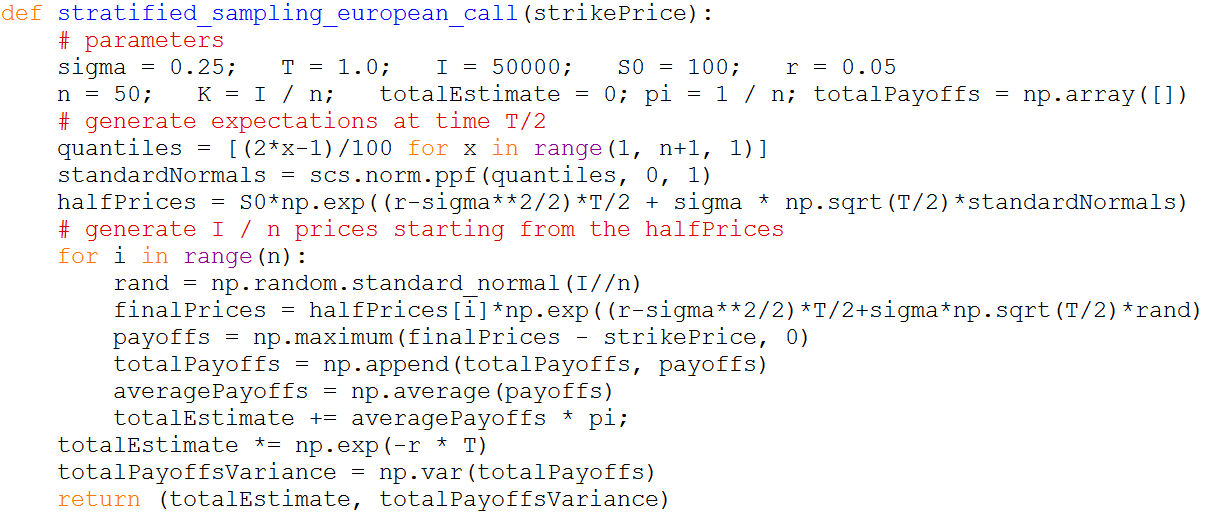
\includegraphics[scale=0.38]{stratified_sampling_european_call_proportional.png}
\end{figure}
\end{frame}

%------------------------------------------------
\begin{frame}
\frametitle{Stratified Sampling - Test}
\begin{figure}[H]
	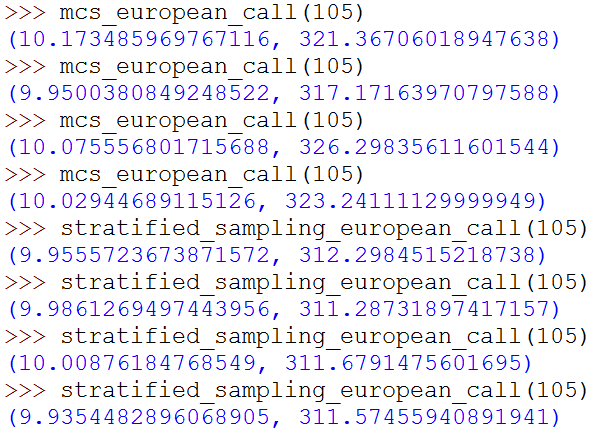
\includegraphics[scale=0.45]{stratified_sampling_european_call_proportional_test.png}
\end{figure}
Although not much, it is clear that there is variance reduction effect.
\end{frame}

\subsection{Importance Sampling}

%------------------------------------------------
\begin{frame}
\frametitle{Importance Sampling - Mathematics}
Importance sampling is a method to reduce variance by changing the probability measure. The word 'Importance' comes from the aim to give more weight to 'important' outcomes by changing measures.\\
We are going to estimate $\alpha = \mathrm{E}[h(X)] = \int h(x)f(x) dx$.\\
In Monte Carlo simulation, $\hat{\alpha} = \hat{\alpha}(n) = \frac{1}{n} \sum_{i=1}^{n} h(X_{i})$\\
By using a change of measure based on the following assumption:
$\forall x \in \mathbb{R}^{d}, f(x) > 0 \implies g(x) > 0$\\
Now the estimate becomes $\alpha = \mathrm{E}[h(X)] = \mathrm{E}[h(X)\frac{f(X)}{g(X)}] = \int h(x)\frac{f(x)}{g(x)} dx$\\
And for simulation, $\hat{\alpha}_{G} = \frac{1}{n} \sum_{i=1}^{n} h(X_{i})\frac{f(X_{i})}{g(X_{i})}$
We are choosing $g$ to make ${X \in A}$ more likely after changing measure.
\end{frame}

%------------------------------------------------
\begin{frame}
\frametitle{Importance Sampling - Mathematics}
In order to reduce variance, we need to implicitly find the $g$ which gives the minimum possible variance. According to the variance formula $\mathrm{Var}(X) = \mathrm{E}(X^{2}) - (\mathrm{E}(X))^{2} $, we have\\
\begin{equation*}
\begin{split}
\mathrm{Var}^{G}[h(X)\frac{f(X)}{g(X)}] &= \mathrm{E}^{G}[h(X)^{2}\frac{f(X)^{2}}{g(X)^{2}}] - (\mathrm{E}^{G}[h(X)\frac{f(X)}{g(X)}])^{2}\\
&= \int \frac{h(x)^{2}f(x)^{2}}{g(x)} dx - (\int \frac{h(x)f(x)}{g(x)}g(x) dx)^{2}\\
\end{split}
\end{equation*}
Here if $h(x) = \frac{g(x)f(x)}{\mathrm{E}(g(x))}$, the variance of estimate will become 0.
\end{frame}

%------------------------------------------------
\begin{frame}
\frametitle{Importance Sampling - Mathematics}
Consider the scenario in which we simulate discrete price paths $S(t_{i}), \forall i = 0, 1, \dots, m$, which is assumed to be a Markov Chain with homogeneous property. Let the continuous transition probability be $f_{i}(S(t_{i-1}),S(t_{i}))$.\\[3mm]
We shall use likelihood ratio $\prod_{i=1}^{m} \frac{f_{i}(S(t_{i-1}),S(t_{i}))}{g_{i}(S(t_{i-1}),S(t_{i}))}$ as risk-neutral measure.
\end{frame}

%------------------------------------------------
\begin{frame}
\frametitle{Importance Sampling - in Black-Scholes World}
\begin{center}
\begin{equation*}
\begin{split}
\mathbb{E}^{\mathbb{Q}}(X) 
&= \int x g(x) dx\\
&= \mathbb{E}^{\mathbb{P}}(\frac{d\mathbb{Q}}{d\mathbb{P}}X) \\
&= \mathbb{E}^{\mathbb{P}}(e^{\lambda W_{T} - \frac{1}{2}\lambda^{2}T}X) \\[7mm]
\end{split}
\end{equation*}
Our aim is to make (where $A>0$)
$$\mathbb{E}^{\mathbb{P}}((S_{T} - K)^{+})= \mathbb{E}^{\mathbb{Q}}(\frac{d\mathbb{P}}{d\mathbb{Q}}(S_{T} - K)^{+}) = \mathbb{E}^{\mathbb{Q}}(e^{((\mu - \frac{\sigma^{2}}{2}+\sigma A)T + \sigma W_{T}^{\mathbb{Q}}})(S_{T} - K)^{+})$$\\[4mm]
Hence $\frac{d\mathbb{Q}}{d\mathbb{P}} = exp\{AW_{T} - \frac{1}{2}A^{2}T\}$
\end{center}
\end{frame}

%------------------------------------------------
\begin{frame}
\frametitle{Importance Sampling - Implementation (buggy)}
\begin{figure}[H]
	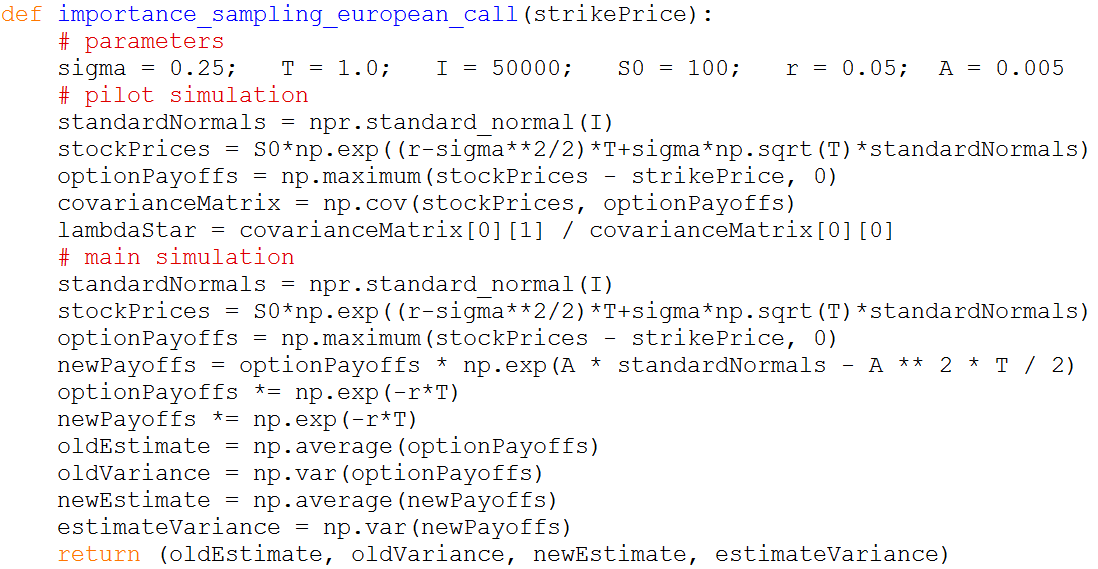
\includegraphics[scale=0.42]{importance_sampling_european_call.png}
\end{figure}
\end{frame}

%------------------------------------------------
\begin{frame}
\frametitle{Put Option Purely Probabilistic Integration - GBM}
Consider the Geometric Brownian Motion model with parameters $r, \sigma, T$, and the strike price $K$ unknown.\\
The expectation of the option payoff can be formulated as:
\begin{equation*}
\begin{split}
\mathrm{E}[X] 
&= \int_{0}^{\infty} max(0, K-x) \mathbb{P}[e^{w} \in dx] \\
&= \int_{0}^{K} (K-x) \frac{1}{\sqrt{2\pi}\sigma\sqrt{T}} \exp\{-\frac{(\ln(x))^{2}}{2T}\} dx\\
&= \int_{-\infty}^{0} (K-e^{x}) \frac{1}{\sqrt{2\pi}\sigma\sqrt{T}} \exp\{-\frac{x^{2}}{2T}\} dx\\
&= \int_{-\infty}^{0} (K-e^{x}) \frac{e^{-\frac{x^{2}}{2T}}}{\sigma\sqrt{2\pi T}} dx\\
&= \int_{-\infty}^{0} K \frac{e^{-\frac{x^{2}}{2T}}}{\sigma\sqrt{2\pi T}} dx - \int_{-\infty}^{0} e^{x} \frac{e^{-\frac{x^{2}}{2T}}}{\sigma\sqrt{2\pi T}} dx\\
\end{split}
\end{equation*}
\end{frame}

%------------------------------------------------
\begin{frame}
\frametitle{Put Option Purely Probabilistic Integration - GBM}
Carry on with the integration
\begin{equation*}
\begin{split}
\mathrm{E}[X] 
&= \int_{-\infty}^{0} K \frac{e^{-\frac{x^{2}}{2T}}}{\sigma\sqrt{2\pi T}} dx - \int_{0}^{\infty} e^{x} \frac{e^{-\frac{x^{2}}{2T}}}{\sigma\sqrt{2\pi T}} dx\\
&= \int_{-\infty}^{0} K \frac{e^{-\frac{x^{2}}{2T}}}{\sigma\sqrt{2\pi T}} dx - \int_{0}^{\infty} e^{-\sqrt{y}} \frac{e^{-\frac{y}{2T}}}{2\sigma\sqrt{y\pi{T}}} dy\\
\end{split}
\end{equation*}
\end{frame}

%------------------------------------------------
\begin{frame}
\frametitle{Call Option Purely Probabilistic Integration - GBM}
Consider the Geometric Brownian Motion model with parameters $r, \sigma, T$, and the strike price $K$ unknown.\\
The expectation of the option payoff can be formulated as:
\begin{equation*}
\begin{split}
\mathrm{E}[X] 
&= \int_{0}^{\infty} max(0, x-K) \mathbb{P}[e^{w} \in dx] \\
&= \int_{K}^{\infty} (x-K) \frac{1}{\sqrt{2\pi}\sigma\sqrt{T}} \exp\{-\frac{(\ln(x))^{2}}{2T}\} dx\\
&= \int_{K}^{\infty} (e^{x}-K) \frac{1}{\sqrt{2\pi}\sigma\sqrt{T}} \exp\{-\frac{x^{2}}{2T}\} dx\\
&= \int_{K}^{\infty} (e^{x}-K) \frac{e^{-\frac{x^{2}}{2T}}}{\sigma\sqrt{2\pi T}} dx\\
&= \int_{K}^{\infty} e^{x} \frac{e^{-\frac{x^{2}}{2T}}}{\sigma\sqrt{2\pi T}} dx - \int_{K}^{\infty} K \frac{e^{-\frac{x^{2}}{2T}}}{\sigma\sqrt{2\pi T}} dx\\
\end{split}
\end{equation*}
\end{frame}

%------------------------------------------------
\begin{frame}
\frametitle{Call Option Purely Probabilistic Integration - GBM}
Carry on with the integration
\begin{equation*}
\begin{split}
\mathrm{E}[X] 
&= \int_{K}^{\infty} e^{x} \frac{e^{-\frac{x^{2}}{2T}}}{\sigma\sqrt{2\pi T}} dx - \int_{K}^{\infty} K \frac{e^{-\frac{x^{2}}{2T}}}{\sigma\sqrt{2\pi T}} dx\\
&= \int_{K^{2}}^{\infty} e^{\sqrt{y}} \frac{e^{-\frac{y}{2T}}}{2\sigma\sqrt{y\pi{T}}} dy - \int_{K}^{\infty} K \frac{e^{-\frac{x^{2}}{2T}}}{\sigma\sqrt{2\pi T}} dx\\
\end{split}
\end{equation*}
\end{frame}

%-----------------------------------------------
\begin{frame}
\Huge{\centerline{Thank You}}
\begin{center}
\begin{normalsize}
\emph{E0007424@u.nus.edu}
\end{normalsize}
\end{center}
\end{frame}

%------------------------------------------------

\end{document} 